%%%%%%%%%%%%%%%%%%%%%%%%%%%%%%%%%%%
%This is the LaTeX ARTICLE template for RSC journals
%Copyright The Royal Society of Chemistry 2016
%%%%%%%%%%%%%%%%%%%%%%%%%%%%%%%%%%%

%\documentclass[twoside,twocolumn,	9pt]{article}
\documentclass[12pt]{article}


\usepackage{extsizes}
\usepackage[super,sort&compress,comma]{natbib} 
\usepackage[version=3]{mhchem}
\usepackage[left=2cm, right=2cm, top=2cm, bottom=3.0cm]{geometry}
%\usepackage[a4paper]{geometry}

\usepackage{balance}
\usepackage{times,mathptmx}
\usepackage{sectsty}
\usepackage{graphicx} 
\usepackage{lastpage}
\usepackage[format=plain,justification=justified,singlelinecheck=false,font={stretch=1.125,small,sf},labelfont=bf,labelsep=space]{caption}
\usepackage{float}
\usepackage{fancyhdr}
\usepackage{fnpos}
\usepackage[english]{babel}
  \renewcommand{\refname}{Notes and references}
\addto{\captionsenglish}{%
}
\usepackage{array}
\usepackage{droidsans}
\usepackage{charter}
\usepackage[T1]{fontenc}
\usepackage[usenames,dvipsnames]{xcolor}
\usepackage{setspace}
\usepackage[compact]{titlesec}
\usepackage{hyperref}
\usepackage[framed]{matlab-prettifier}
\usepackage{caption}
\usepackage{float}
\usepackage{wrapfig}
\usepackage{multicol}
\usepackage{tikz}
\usetikzlibrary{calc}
\usetikzlibrary{decorations.pathmorphing}

\newcommand{\Matlab}{\textsc{Matlab}}

%%%Please don't disable any packages in the preamble, as this may cause the template to display incorrectly.%%%


\usepackage{epstopdf}%This line makes .eps figures into .pdf - please comment out if not required.

\definecolor{cream}{RGB}{222,217,201}
%%%%%%%%%%%%%%%%%%%%%%%%%%%%%%%%%%%%%%%%%%%%%%%%%%%%%%%%%%%%%%%%%
\begin{document}


\begin{titlepage}
	\newgeometry{left=1cm, right=2cm, top=1cm, bottom=3.0cm}
	
	\begin{multicols}{2}
		
	
	\begin{flushright}
	
		
		
		
		
		\vspace*{4cm}
		%\hspace{4cm}
		
		\textbf{\\ Practical Report\\}
		\vspace*{5cm}
		ON\\
		\vspace{1cm}
		%\hspace{6cm}
		\textbf{\huge
			LINEAR MODEL OF \\
		\vspace{0.33cm}
			THE
			 DC MOTOR
		}
		
		\vspace{0.5cm}
		
		 \textrm{WRITTEN BY:\\
		 	\textbf{Grover Aruquipa\\
		 	}\\
	 		\vspace*{1 cm}
	 	\textrm{ No:\\
	 		\textbf{3540901/01701} \\
		 }}	
		 \vspace*{1 cm}
	 	\makebox{}\\
		 \textbf{Mathematical Modeling and simulation}
		\vspace{0.8cm}
		
		
			%\centering
		
		\makebox{}\\
		October 15, 2020
		
	\end{flushright}

	\end{multicols}

\end{titlepage}
\restoregeometry

\newpage

\pagestyle{fancy}
\thispagestyle{plain}
\fancypagestyle{plain}{

%%%HEADER%%%
%\fancyhead[C]{\includegraphics[width=18.5cm]{head_foot/header_bar}}
%\fancyhead[L]{\hspace{0cm}\vspace{0.5cm}\includegraphics[height=30pt]{head_foot/header1.jpg}}
%\fancyhead[R]{\hspace{0cm}\vspace{0.7cm}\includegraphics[height=55pt]{head_foot/spb1.jpg}}
\renewcommand{\headrulewidth}{0pt}
}
%%%END OF HEADER%%%

%%%PAGE SETUP - Please do not change any commands within this section%%%
\makeFNbottom
\makeatletter
\renewcommand\LARGE{\@setfontsize\LARGE{15pt}{17}}
\renewcommand\Large{\@setfontsize\Large{12pt}{14}}
\renewcommand\large{\@setfontsize\large{10pt}{12}}
\renewcommand\footnotesize{\@setfontsize\footnotesize{7pt}{10}}
\makeatother

\renewcommand{\thefootnote}{\fnsymbol{footnote}}
\renewcommand\footnoterule{\vspace*{1pt}% 
\color{cream}\hrule width 3.5in height 0.4pt \color{black}\vspace*{5pt}} 
\setcounter{secnumdepth}{3}

\makeatletter 
\renewcommand\@biblabel[1]{#1}            
\renewcommand\@makefntext[1]% 
{\noindent\makebox[0pt][r]{\@thefnmark\,}#1}
\makeatother 
\renewcommand{\figurename}{\small{Fig.}~}
\sectionfont{\sffamily\Large}
\subsectionfont{\normalsize}
\subsubsectionfont{\bf}
\setstretch{1.125} %In particular, please do not alter this line.
\setlength{\skip\footins}{0.8cm}
\setlength{\footnotesep}{0.25cm}
\setlength{\jot}{10pt}
\titlespacing*{\section}{4pt}{4pt}{4pt}
\titlespacing*{\subsection}{2pt}{15pt}{1pt}
%%%END OF PAGE SETUP%%%

%%%FOOTER%%%\fancyfoot{}
\fancyfoot{}
%\fancyfoot[LO,RE]{\vspace{-7.1pt}\includegraphics[height=9pt]{head_foot/LF}}
%\fancyfoot[CO]{\vspace{-7.1pt}\hspace{13.2cm}\includegraphics{head_foot/RF}}
%\fancyfoot[CE]{\vspace{-7.2pt}\hspace{-14.2cm}\includegraphics{head_foot/RF}}
%\fancyfoot[RO]{\footnotesize{\sffamily{1--\pageref{LastPage} ~\textbar  \hspace{2pt}\thepage}}}
%\fancyfoot[LE]{\footnotesize{\sffamily{\thepage~\textbar\hspace{3.45cm} 1--\pageref{LastPage}}}}
\fancyfoot[RO, LE] {\thepage}
\fancyhead{}
\renewcommand{\headrulewidth}{0pt} 
\renewcommand{\footrulewidth}{0pt}
\setlength{\arrayrulewidth}{1pt}
\setlength{\columnsep}{6.5mm}
\setlength\bibsep{1pt}

%%%END OF FOOTER%%%

%%%FIGURE SETUP - please do not change any commands within this section%%%
\makeatletter 
\newlength{\figrulesep} 
\setlength{\figrulesep}{0.5\textfloatsep} 

\newcommand{\topfigrule}{\vspace*{-1pt}% 
\noindent{\color{cream}\rule[-\figrulesep]{\columnwidth}{1.5pt}} }

\newcommand{\botfigrule}{\vspace*{-2pt}% 
\noindent{\color{cream}\rule[\figrulesep]{\columnwidth}{1.5pt}} }

\newcommand{\dblfigrule}{\vspace*{-1pt}% 
\noindent{\color{cream}\rule[-\figrulesep]{\textwidth}{1.5pt}} }

\makeatother
%%%END OF FIGURE SETUP%%%

%%%TITLE, AUTHORS AND ABSTRACT%%%
%\twocolumn[
  %\begin{@twocolumnfalse}
\vspace{3cm}
\sffamily
\begin{center}
\LARGE{\textbf{LINEAR MODEL OF THE DC MOTOR}} \\%Article title goes here instead of 	
\end{center}

\normalsize{\textbf{Abstract}\\
In this document is analyzed the behavioral for a a linear motor using techniques controls to understand the stability implemented with \Matlab. } \\%The abstrast goes here instead of the text "The abstract should be..."

 %\end{@twocolumnfalse} \vspace{0.6cm}

 % ]
%%%END OF TITLE, AUTHORS AND ABSTRACT%%%

%%%FONT SETUP - please do not change any commands within this section
\renewcommand*\rmdefault{bch}\normalfont\upshape
\rmfamily
\section*{}
\vspace{-1cm}


%%%FOOTNOTES%%%

%\footnotetext{\textit{$^{b}$~Peter the Great St Petesburg Polytechnic University, Russia, Saint Petesburg. }}
%\footnotetext{\dag~Laboratory 1 from the subject mathematical modeling and simulation to the Master Program Intelligent Systems}

%Please use \dag to cite the ESI in the main text of the article.
%If you article does not have ESI please remove the the \dag symbol from the title and the footnotetext below.




%%%END OF FOOTNOTES%%%

%%%MAIN TEXT%%%%
\textbf{}\setcounter{page}{1}
\section{Introduction}
In this report is analyzed the behavioral from the model of a Linear model of the DC motor, so that is present the results from a simulation implemented with \Matlab, in the first part is analyzed the equations from the model, in the state of space and in the space of frequency, after of that we show the code and the results with a step, the bode diagram and the Nyquist diagram to the end is presented a discussion and a conclusion about the results.
\section{Lineal model from the DC motor}
In this laboratory is analyzed the next differential equation:

\begin{equation}
U_{M}=R_{\alpha}I_{\alpha}+K_{e}W+L_{\alpha}\dfrac{dI_{\alpha}}{dt}
\end{equation}
\begin{equation}
J\dfrac{dW}{dt}=M-M_{L}
\end{equation}
Where $U_{M}$ is the voltage of the motor[V], $I_{a}$ is the motor armature current[A], $W$ is the motor speed(angular velocity)[rad/sec], $E_a$ is electromotive force[V], $J$ is a moment of inertia$kgm^{2}$ and $M_{L}$ a torque for external load [Nm].\\
So that in other form is possible have the next system:
\begin{equation}
\begin{cases}
\dfrac{dI_{\alpha}}{dt}=\dfrac{1}{L_{\alpha}}(-R_{\alpha}I_{\alpha}-K_{e}W+U_{M})\\
\dfrac{dW}{dt}=\dfrac{1}{J}(K_{W}I_{\alpha}-M_{L})
\end{cases}
\end{equation}
Where $T_{\alpha}=\dfrac{L_{\alpha}}{R_{\alpha}}$ is the electrical time constant, [s], $T_{M}=\dfrac{JR_{\alpha}}{K_{e}K{m}}$ [s], so that the (3) could be expressed in the frequency state:\\
\begin{equation}
W_{M}(s)=\dfrac{W(s)}{U_{M}(s)}=\dfrac{1/K_{e}}{T_{m}T_{a}s^{2}+T_{m}s+1}
\end{equation}
So that with the equation (4) is possible use to analyze the dynamic from the system.
\section{Cases to analyze}
After obtaining the Linear model expressed in the Frequency state is proposed analyze different types of motors and their parameters, so that is extracted the next table from the motors :
\begin{center}
\renewcommand{\arraystretch}{1.5}
\begin{tabular}{|c|c|c|c|}
	\hline
	Parameter&(A-MAX 22-110149)& (A-MAX 22-110150)& (A-MAX 22-110152) \\
	\hline
	Terminal resistance [$\omega$]& 9.09 &14  &  33.3\\
	\hline
	Terminal inductance [$mH$]&0.585  & 0.891 & 2.1 \\
	\hline
	Inv. of Speed const. [$\frac{V}{rad\cdot s^{-1}}$]&$13.9\times 10^{-3}$  & $17.1\times 10^{-3}$ &$26.2\times 10^{-3}$  \\
	\hline
	Rotor Inertial[$kgm^{2}$]& $4.2 \times 10^{-7}$ & $4.13\times 10^{-7}$ &$4.09\times 10^{-7}$  \\
	\hline
\end{tabular}
\end{center}
And the next condition are necessary for the analyze of the model:

\begin{center}
	$K_{m}=K_{e}$\\
	$T_{a}=\dfrac{L_{a}}{R_{a}}$\\
	$T_{m} = JR_{a}/(K_{e}*K_{m})$ 

\end{center}

With the last algebraically expression and the table of parameters is possible analyze the behavioral of  motors using the equation (4).


\section{Implementation}
So that in the next code is implemented the equation (4) and analyzed the response with a step, impulse, the bode diagram in the different cases and the Nyquist diagram:\\
%\newgeometry{left=1.5cm, right=1.5cm, top=1.785cm, bottom=3.0cm}

\lstinputlisting[style=matlab-editor,caption={Code from \Matlab}]{code.m} 

\section{Results}
In this section is presented the results from the experiment the linear system.
\subsection{Nyquist Diagram}
The Nyquist diagram help to show the stability from the system then we need consider the point (-1,0) to have a perspective about the stability from the system, so that in the figure 1 is presented the three cases proposed. Is observable how this point is not in the area from the curve, then the means is the system don't is stable with a open loop.
\begin{figure}[H]
\centering		
		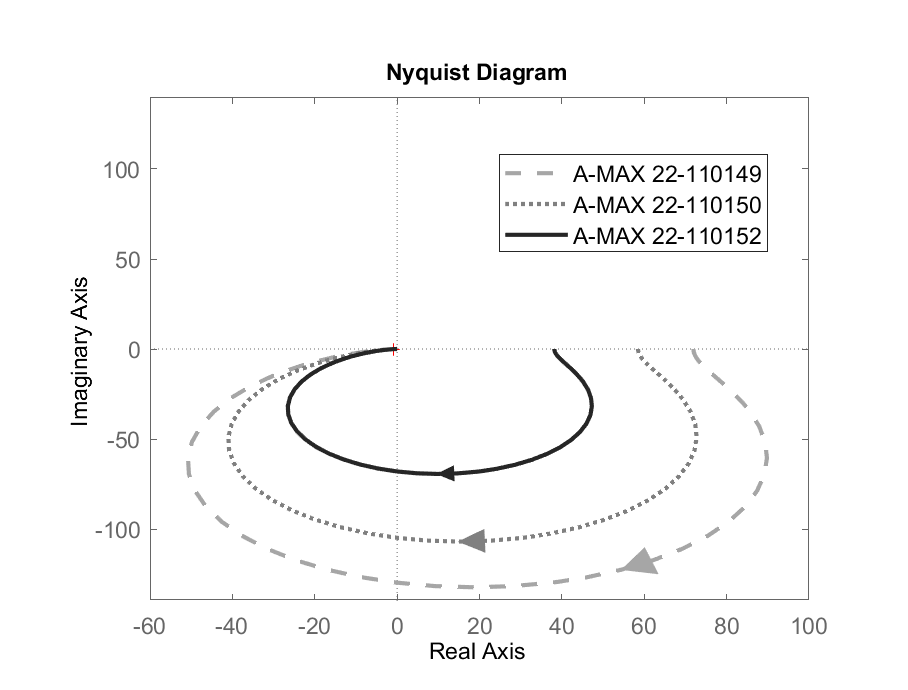
\includegraphics[scale=0.8]{nyquist.eps}
		\captionsetup{justification=centering}
		\caption{Nyquist diagram for the system.}
		\label{f1}
	%\end{center}
\end{figure}

\subsection{Bode diagram}
In this case in the figure 2 Bode helps to provide a quickly stability criteria,so that is necessary observe how to $motor1$ the phase margin is 3.77 $[s]$, to $motor$ the phase margin is similar to 3.77 $deg$ and to motor3 the phase margin is to the same case similar to 3.77$deg$ another important information is how the phase never crosser with 180 deg and the means is the gain margin is too high, so that with this graphic is necessary use root locus in order to optimize the stability from the system.

\begin{figure}[H]
	\centering		
	\includegraphics[scale=0.3]{bode.eps}
	\captionsetup{justification=centering}
	
	\caption{Bode diagram for the system.}
	\label{f2}
	%\end{center}
\end{figure}

\subsection{Impulse Response}
The impulse response or Dirac Delta Input helps to understand the behavior from the system with a high and quickly excitation then in this case the graph show how to the case from $motor2$ the system is unstable before 600-1400 of amplitude which means in a real system can be translated to instability or failures by the high amplitude and the over damping, then in the case form $motor1$and $motor3$ the answer have a high setting time and in a personal observation this type of signal not necessarily good in real time systems, so is necessary a synchronization.

\begin{figure}[H]
	\centering		
	\includegraphics[scale=0.3]{impulse.eps}
	\captionsetup{justification=centering}
	\caption{Impulse response.}
	\label{f3}
	%\end{center}
\end{figure}
\subsection{Step Response}
\begin{figure}[H]
	\centering		
	\includegraphics[scale=0.3]{step_Response.eps}
	
	\captionsetup{justification=centering}
	
	\caption{Step response.}
	\label{f3}
	%\end{center}
\end{figure}
The step response to the system have a interesting answer, the most relevant response is from the case $motor11$ the overshoot is not too high respect with the other cases,but the rise time could be better, in the case from $motor2$ and $motor3$ the problems is a high overshoot and a high rise time. 

\section{Conclusion}
To conclude the response of the three previously proposed cases is observed, then according to the stability and response graphs of the system for an impulse signal and step type it is necessary to perform a closed loop and tuning to optimize the response of the system in this way this laboratory served to observe the behavior of open loop systems and in the same way in the future it is necessary to apply a control system to have a better system response



\end{document}
